% Created 2018-10-22 Mon 21:00
% Intended LaTeX compiler: pdflatex
\documentclass[11pt]{article}
\usepackage[utf8]{inputenc}
\usepackage[T1]{fontenc}
\usepackage{graphicx}
\usepackage{grffile}
\usepackage{longtable}
\usepackage{wrapfig}
\usepackage{rotating}
\usepackage[normalem]{ulem}
\usepackage{amsmath}
\usepackage{textcomp}
\usepackage{amssymb}
\usepackage{capt-of}
\usepackage{hyperref}
\author{Kai Lukowiak}
\date{\today}
\title{Gas Price Micro Markets}
\hypersetup{
 pdfauthor={Kai Lukowiak},
 pdftitle={Gas Price Micro Markets},
 pdfkeywords={},
 pdfsubject={},
 pdfcreator={Emacs 26.1 (Org mode 9.1.9)}, 
 pdflang={English}}
\begin{document}

\maketitle
\begin{abstract}

Gas station prices are highly dependent on competiton. Due to the nature of gasoline
markets this competition is very local. Industry is not very sophisticated in
segmenting these micro-markets leaving money on the table.

This proposal shows the roadmap to use variation and similarity in regional prices
and geospatial data to identify these micro-markets and find outliers that are
close to but otherwise perform differently.

The end goal is to provide information on these stations along with a framework
that companies can use to experiment further.

With proprietary data, this could be turned into an optimization problem,
however, given that I can only use public data, the problem is one of unsupervised
learning, specifically clustering. I will use the relationship between pure
geographic clustering and clustering based on geography and margin correlation.
This has the benefit of creating a quasi supervised learning environment.

\end{abstract}

\section{Description of the Problem}
\label{sec:org16d72e9}
Retail Gas Prices (RGP) are determined in the competitive market. Gas stations
are surprisingly unsophisticated given that the market in Canada is \href{https://www.ibisworld.ca/industry-trends/market-research-reports/retail-trade/gas-stations.html}{\$34 billion}.
If pricing is granular to the site level, it is almost entirely set by regional
or even station managers and national campaigns do not have the granularity to
capitalize on market differences. Companies that set prices at corporate offices
or have corporate involvement in setting daily prices use \href{https://www.gasbuddy.com/}{GasBuddy}, or GasBudy
supplimented data.

There are many facets that go into the definition of a competitive market.
Cataloguing all features and recording them is a gargantuan task. Instead this
study hopes to discern which stations may be different from their surrounding
competition. This will be done my comparing a demeaned marginal price.


The competition is based on many factors like loyalty programs, marketing,
customer preferences etc. One major influence on RGP is geographic
location. Even within the same distribution market (same base fuel price), a
station on a major highway, one in close proximity to three other competitors
and one in a rural area will all behave differently.

Segmenting these markets to understand stations direct competitors is key to
maximizing profit.

\section{Why the problem is interesting}
\label{sec:orga9f4d0a}

There is aproximetly \href{https://www150.statcan.gc.ca/t1/tbl1/en/tv.action?pid=2310006601}{\$50 billion L} of motor fuels sold in Canada yearly.
\(\50,000,000,000L \cdot \alpha\) where \(\alpha\) is small increase in cents per
litre (CPL) is still a lot of money. 

Beyond the fiscal incentives, this is an interesting study because it will
reveal (hopefully) two findings. The first is finding relevant markets in
geographic areas. For example, it is easy to believe that gas stations on
different sides of a major river or other barrier would price differently.

Secondly, after geographic markets are found, gas stations that are contained
within a similar geographic area, but that price differently can be further
analyzed. For example, a suburban area may be a well defined market with similar
price fluctuation in stations except for one. This will allow an analyst to
further investigate this one station to find which features make it more
profitable (or less).

These findings could help set prices more efficiently as well as indicate which
areas are best for future investment. 


\section{What other approaches have been tried}
\label{sec:org403c263}

Investigating retail gasoline markets is nothing new. Most recently in Canada,
\href{https://www.parkland.ca/en/our-businesses/retail/}{Parkland} has a large market of retail stations and merged with \href{https://en.wikipedia.org/wiki/Pioneer\_Energy}{Pioneer Energy}
based in Ontario.  The \href{http://www.competitionbureau.gc.ca/eic/site/cb-bc.nsf/eng/04053.html}{Competition Bureau} forced Parkland to divest several
stations they believed would form regional monopolies.

I am also sure marketing departments have segmented promotional efforts based on
location.

Both of these focus on a more macro level geography. Or, if they do look at
micro geography, only do so in specific areas like a small town where 2/3 gas
stations will merge.

There are many examples of spatial/temporal regression investigating gas prices
in the economic literature. Some of these are quite granular, although I was
unable to find any on the same scale as I plan. These are listed in the links
at the bottom of this paper.

Further these look at the causal effect of distance on price. My intention is to
cluster sites and compare them to other clustering techniques such as
KNN or K-Means. Some examples of spatial regression can be seen below as well.


\section{Discussion on your hypothesis is and how your specific solution will improve}
\label{sec:orgb20edd6}

My hypothesis is that there are anomalous gas stations and unobserved
sub-regions which can be detected through variance spatial/temporal analysis.

Further, due to my disinterest in causality/interpretation I can use also use
non-linear techniques that make interpretation difficult.

I plan on using four approaches to solve this. 

\subsection{PySal}
\label{sec:orgcff813b}
My first approach will be to use \href{https://www.earthdatascience.org/tutorials/intro-to-spatial-regression/}{PySal} to investigate linear relationships
between stores and cluster them by similarity to their prices.

\subsection{Weighted Leas Squares}
\label{sec:orgf14c874}
Secondly, I also plan on investigating other correlation/regression techniques with
numbers weighted by distance. For example, using an exponential decay function
to weight to competitors based on distance.

\subsection{K-Means (Weighted)}
\label{sec:org3169899}
Thirdly, I will use clustering algorithms (K-Means) to cluster stations based on
geography. This will be done using a vector of different centroids (eg: 6:100).
This will form clusters based on the shortest geographical distance. These
geo-clusters will be used to tune the clusters that use margin data.

Classic clustering algorithms rely on scaled variables. For example, clustering
people based on gender, income, age and education requires that all variables
have a mean of zero and unit standard deviation. If I were to do that with the
lat/lng variables and margin, margin would have a very overstated impact because
the lat/lng features span thousands of killometres and margins are generally
between -2 and 10. Thus, I have to decrease the impact of this. 

\href{https://pdfs.semanticscholar.org/77e7/55fba9432219dba7bd83302044f2e86e5056.pdf}{This} paper has some interesting results on spatial clustering.


There are a few possible approaches. I can segment each city on it's own so that
the variance in distance is less. I can also reduce the impact of margins by
multiplying them by a fraction and comparing how closely the results aligned to
the pure geo-clusters. This fraction would need to be tuned so that no site was
no further away than the second closest centroid. More experimentation is needed
to fine tune this. 

An other possible approach would be increase the parameter on the margin feature
until just before a station is contained in a closed set of two other locations
in another set. For example:

\begin{center}
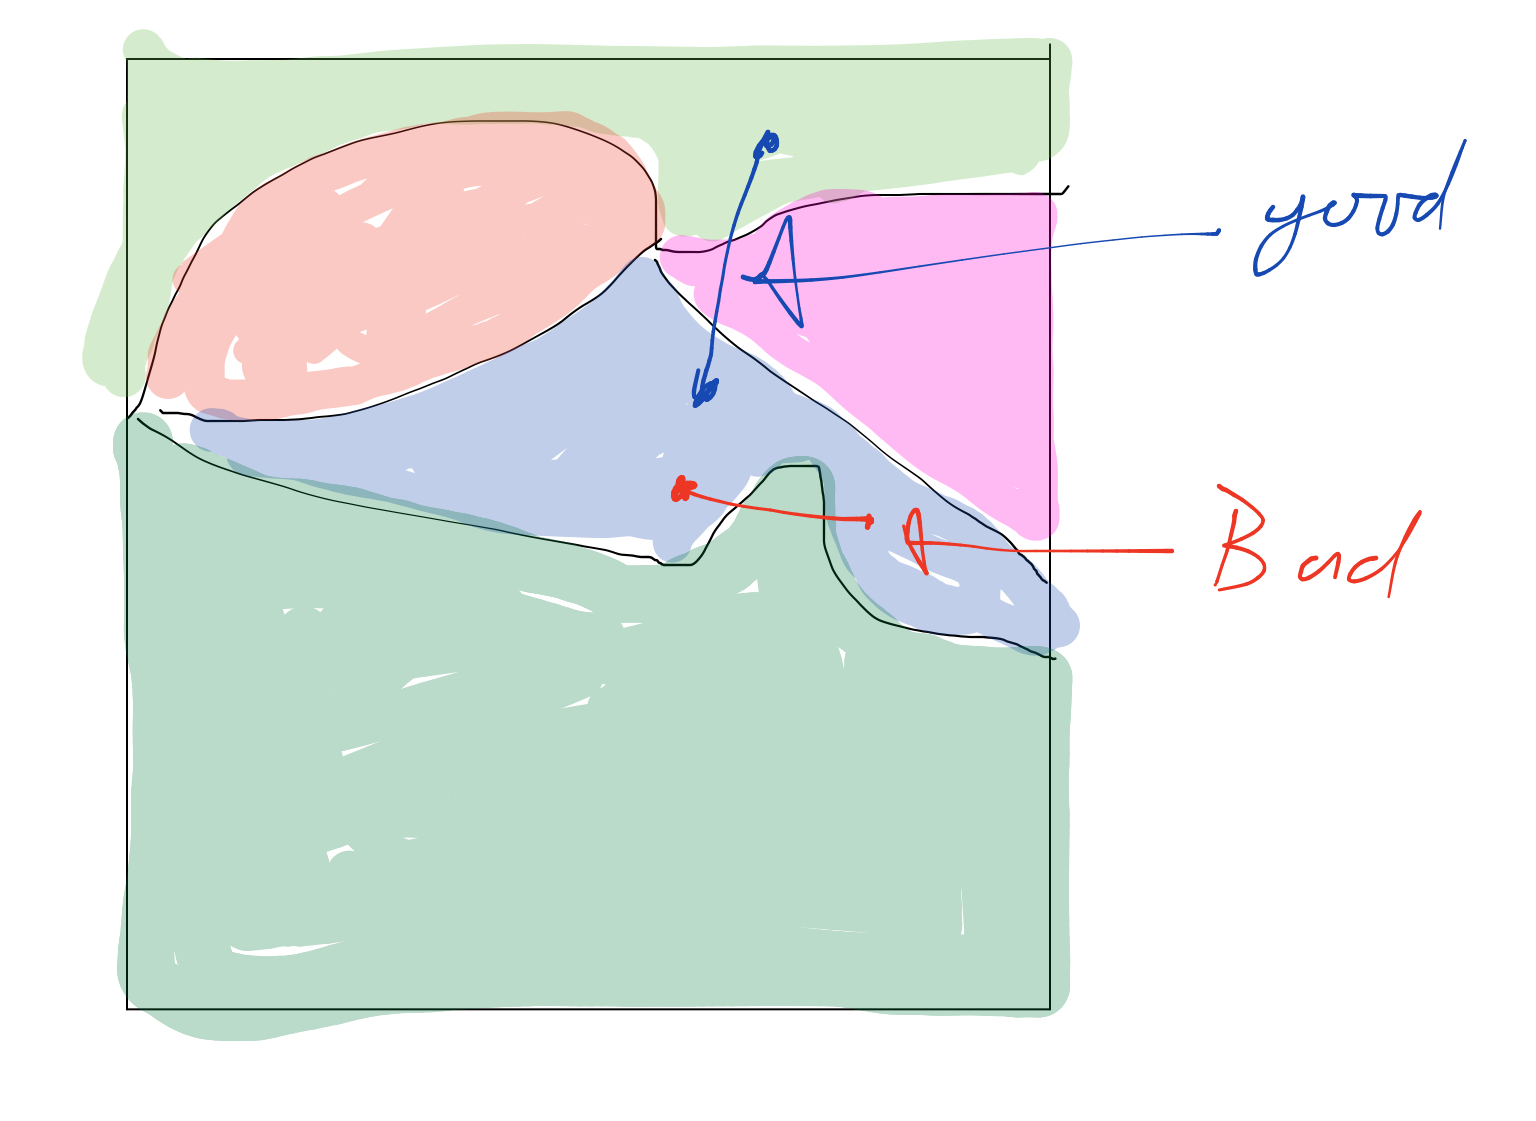
\includegraphics[angle=0,width=15cm]{./img/IMG_0147.jpg}
\end{center}

That is, the green site in the blue area (peninsula) can be crossed by two sites
in blue. The pink set between the blue and green is totally fine.


\subsection{KNN}
\label{sec:org6972356}

Fourthly, I will try a KNN approach. A KNN regression might be very interesting
from a predictive point of view for any particular gas station so I will report
the results, but this won't help us out with finding regions. To find regions we
must use KNN as a classifier. Therefore, we need to lable the data. To do this I
will use K-Means to classify the margins, most likely by city. I will then train
a KNN model to clasify these. For example, if we were looking for low, medium,
and high margin areas, we would lable each individual gas station and then train
the KNN to clasify these. Once the model was trained, the areas can be plotted.


I think the results of the KNN will be most interesting and applicable as they
have the clearest path to success and minimal model tuning. This also solves the 
problem with un-supervised learning as I'm basically just binning the margins.

\section{Issues}
\label{sec:org672fee8}

I faced several data aquasition issues including malfunctioning servers. I've
set up warning systems to notify me if it stops working but the cron job is
still not functioning perfectly. 

I am also finding it harder to create visualization of maps in python. I've thus
switched my EDA over to R, however, I didn't have time to come up with anything
good enough to incldue here.

While many of my approaches are rather experimental or untested, I feel confident
in my KNN approach that I will get something interesting. 

\section{Effects of Edgeworth Cycles}
\label{sec:orgf0006e6}

\href{https://en.wikipedia.org/wiki/Edgeworth\_price\_cycle}{Edgeworth Price Cycles} occur in competitive industries where firms find it
profit maximizing to cut prices until they reach marginal cost. At this point,
they can profit maximize by increases prices well above marginal cost. This
cycle repeats, and in the case of retail gas, often on a weekly basis. I plan on
using this cycle to determine relevant markets. 

\section{Additional Features}
\label{sec:org9cce275}

Weather, day of week, month of year, holidays and area income all play a role in
demand for gasoline. After taking out the tax and rack (manufacturer price) for
the gasoline I will regress price on these variable, along with possible lags
to. I will then take the residuals from this regression and use them in my
models.


\section{Data Acquisition}
\label{sec:org068b4e4}

I have a script scraping GasBuddy for 6 cities in Western Canada. While I have
had some issues with my server functioning, it is getting more robust. 

I've also been able to connect to a weather API. I use google maps API to scrape
latitude and longitude for each station. I also use Governmental sources to get
the Rack price.

\section{Aditional Steps}
\label{sec:org91d2ac0}

My goal is to have this used in industy. Here is a short outline of one possible
use case.

For each store that a company owns, they can find the relevant micro-market
through one of the algorithms.

After this is determined, the firm should regress their price, competitors prices,
and other features on their own volume. This will show how much volume they will
lose by raising their prices over their competition, or gain volume by having a
lower relative price.

The firm should then take their proprietary margin information and take the
derivative of their profit equation WRT the price difference:

$$
Profit = (Price - Margin) * f(Price_{firm}, Price_{competitors}, v)
$$

where \(v\) is any other feature. 

The firm should then set this to zero and solve for the price.

\section{Additional Info}
\label{sec:orgfb1fe8e}

\begin{itemize}
\item \url{https://link.springer.com/article/10.1007/s00168-007-0206-7}
\item \url{https://www.jstor.org/stable/20111978?read-now=1\&googleloggedin=true\&seq=1\#page\_scan\_tab\_contents}
\item \url{https://link.springer.com/chapter/10.1007/978-3-7908-2070-6\_12}
\item \url{http://journals.ama.org/doi/abs/10.1509/jmkr.44.4.622?code=amma-site}
\item \url{https://www.jstor.org/stable/41323223?seq=1\%23page\_scan\_tab\_contents}
\item \url{http://ses.wsu.edu/wp-content/uploads/2015/03/SpatialDifferences.pdf}
\item \url{http://www.econ.uiuc.edu/\~lab/workshop/Spatial\_in\_R.html}
\item \url{http://darribas.org/gds\_scipy16/ipynb\_md/08\_spatial\_regression.html}
\end{itemize}
\end{document}
